\documentclass[../rzero]{subfiles}
\begin{document}
\chapter{Physics Today}\label{physicsTodayChapter}

\begin{chapquote}{Lord Kelvin}
``In science there is only physics; all the rest is stamp collecting.''
\end{chapquote}





\section{Stamp Collecting}
Collecting stamps in physics consists of interpreting every experimental result as another stamp of approval. Why is no one worried about:
\begin{figure}
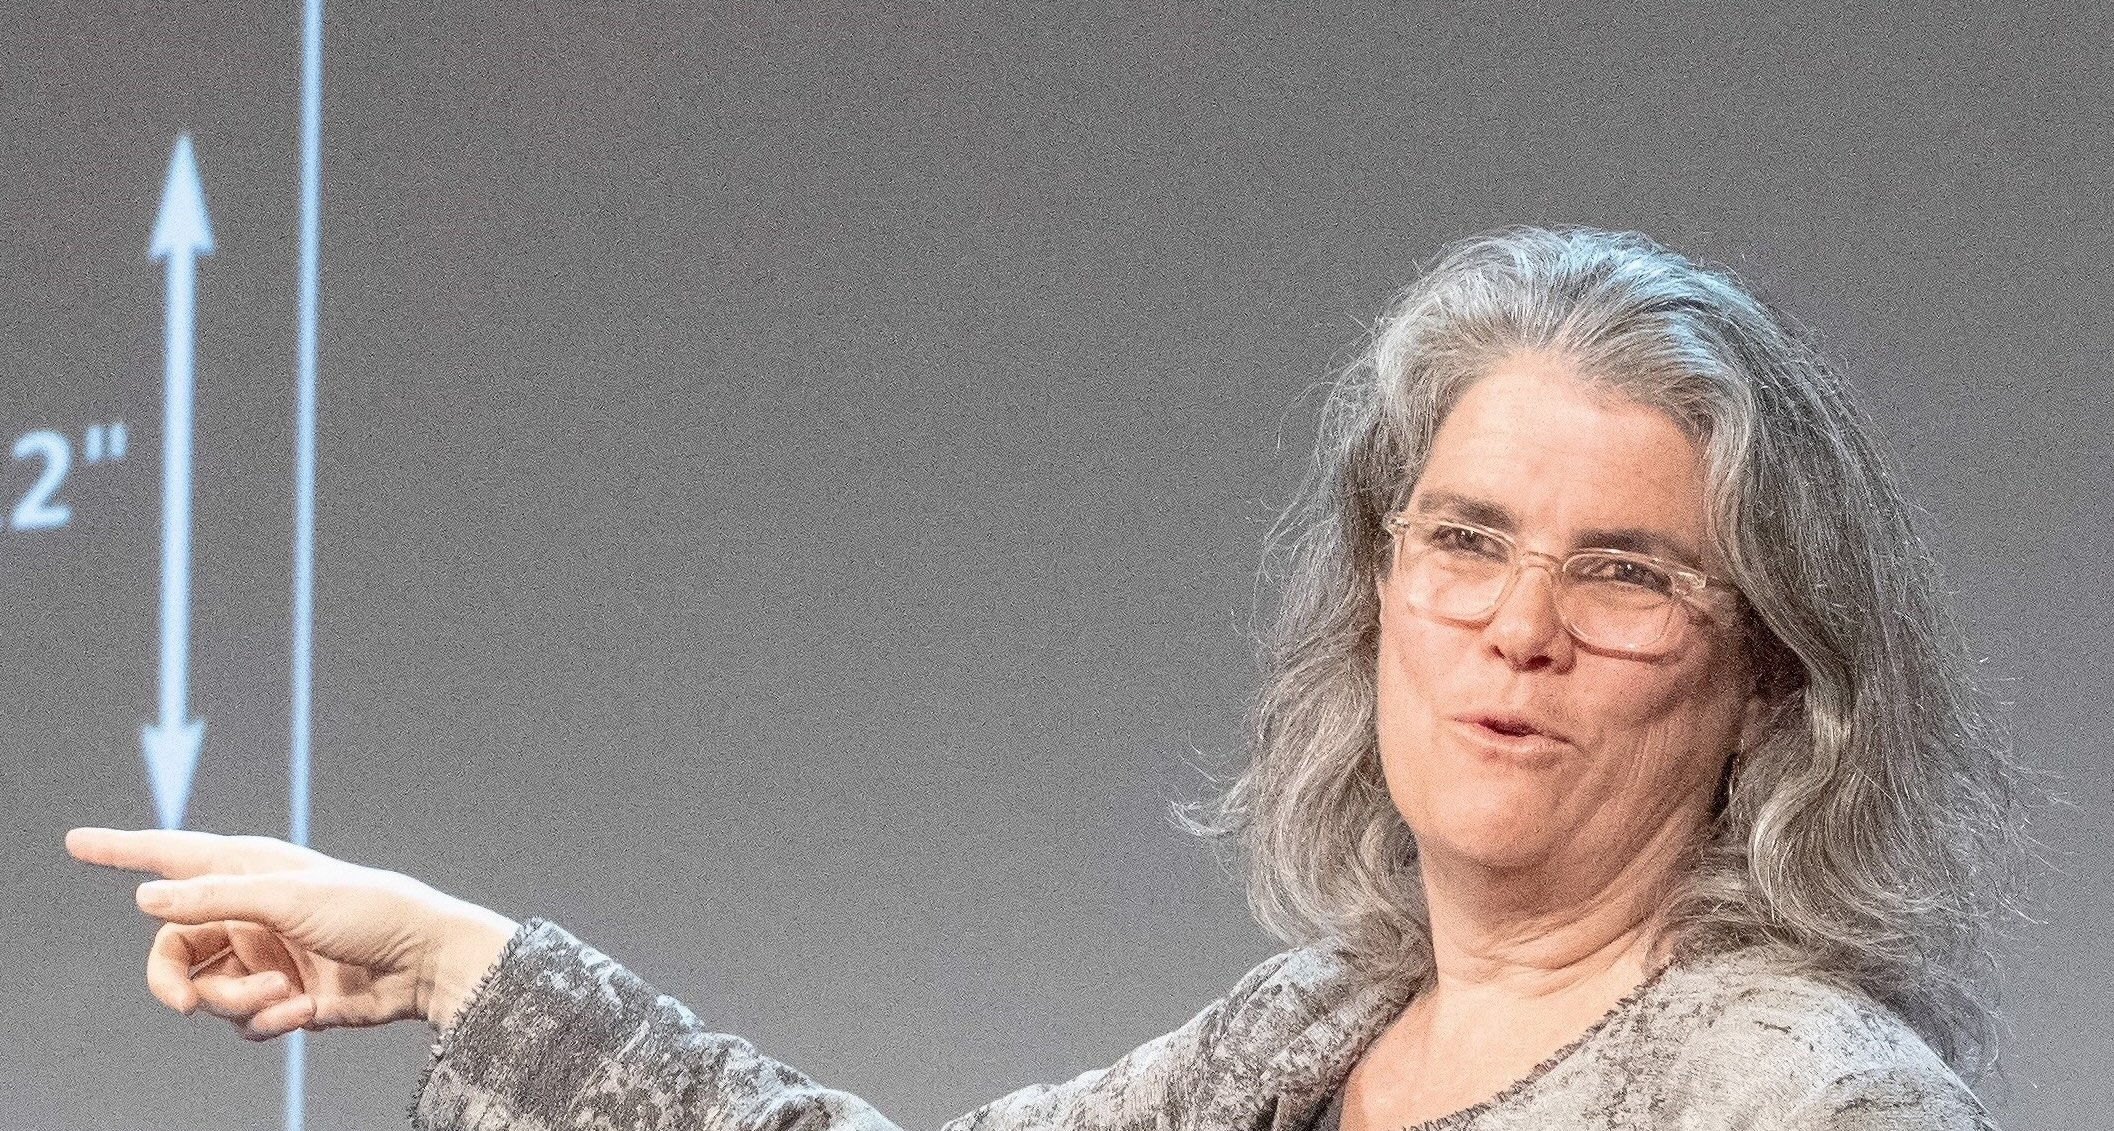
\includegraphics[width=0.65\textwidth]{chapters/images/andrea-ghez.jpg}
\caption{"for the discovery of a supermassive compact object at the centre of our galaxy"   From\cite{borderlinerebelEnglishAndreaGhez2019} Creative Commons}
\label{andrea-ghez}
\end{figure}

\begin{itemize}
  \item Forty free parameters in the Standard Model.
  \item No cool hairdos anymore.\footnote{appears fixed. see Figure (\ref{andrea-ghez}) Thanks!}
  \item Dark Matter completely missing in the Standard Model.
  \item Dark Energy completely missing in the Standard Model.
  \item String Theory$^{TM}$.
  \item Dippy renormalization in QED.
  \item Completely unrenormalizable strong force.
  \item Completely ungovernable strong force.
  \item Completely unmanageable strong force.
  \item No coherent model of the vacuum.
  \item 1000 person years on Quantum Gravity/Strings/Loops and not much progress.
  \item Astronomy kicking its butt.
  \item Global schools of thought built using social media.
  \item Independent free thought.
  \item 2024 Nobel doesn't even go to a physicist.
  \item 27 Dimensions.
  \item 11 Dimensions.
  \item Heck, 5 dimensions.
  \item Infinite multiverses (at least 3).
  \item iPhones are cool, but we don't have flying cars.
  \item Jillions of bandwagon papers. :-(
\end{itemize}

\section{Rant}
Obviously physics is filled with mostly nice people. Wouldn't want to ruffle any feathers.

Theoretical physics went well until about 1980. Theoretical physics then stumbled. Two things happened. Firstly, the model of nature that was settled on around that time, the Standard Model, has gone from explaining virtually everything in the world to about 3-5\% of it. Extensions to that theory, primarily, Super Symmetry, String Theory, and Loop Quantum Gravity have proved unfruitful to say the least. \cite{woit2007not}\cite{smolin2007trouble}\cite{hossenfelder2018lost}. But perhaps the biggest problem are the top end schools of thought themselves. Only a few lines of thought have been permitted at all, and if 10,000 person years of effort are any indication, these directions are not useful. 

\subsection{How do we Restart Physics?}
I don't know. But maybe we need to break it, and see what happens.
\subsection{Books}
\begin{itemize}
  \item Lost in Math.
  \item Not Even Wrong.
  \item Not this Book. (how is that working out?)
  \item Lee Smolin
  \item For some reason I'm not gonna list actual great useful works that allow actual calculations so we can actually move ahead. But these do exist! Know your stuff.
\end{itemize}

We should watch:
\begin{itemize}
  \item Youtube videos by Dialect.
  \item Pisra.org videos.
  \item Channels
  \item Nice Guy daily
  \item ....OTHERS
\end{itemize}

\section{Summary}
Do everything I wouldn't do. 


\end{document}
